\documentclass[sigconf, nonacm]{acmart}

\def\BibTeX{{\rm B\kern-.05em{\sc i\kern-.025em b}\kern-.08emT\kern-.1667em\lower.7ex\hbox{E}\kern-.125emX}}

\copyrightyear{2019}
\acmYear{2019}

\usepackage[]{algorithm2e}

\begin{document}

\title{Fair ranking in academic search}
\subtitle{Notebook for the TREC 2019 Fair Ranking Track}


\author{Malte Bonart}
\email{malte.bonart@th-koeln.de}
\orcid{0000-0001-9548-9918}
\affiliation{%
  \institution{Technische Hochschule Köln}
}


\begin{abstract}
This notebook summarizes our participation in the first Fair Ranking Track at TREC 2019 \cite{asia_biega_trec_2019}. We shortly introduce the problem setting, give an overview of the software framework, and discuss the task and the results of our two submissions.  
\end{abstract}

\keywords{ranking, algorithmic fairness, learning-to-rank}

\maketitle

\section{Introduction}

The issue of algorithmic fairness has recently gained popularity in the IR community \cite{ekstrand_fairness_2019, castillo_fairness_2019}. In this year's Fair Ranking Track, the goal was to re-rank rankings of scholarly articles from a productive academic search engine such that groups of authors are 'fairly' exposed in the sequence of rankings. The data for this challenge was taken from the \emph{SemanticScholar} open research corpus that contains around 47 million articles \cite{ammar_18}. 

It was assumed, that a fair exposure for a group of authors was satisfied if the group's $g$ share of aggregated exposure $\mathcal{E}_g$ equals a group's share of aggregated relevance $\mathcal{R}_g$, such that

\begin{equation}
    \mathcal{E}_g = \frac{\sum_{a \in \mathcal{A}_g}\sum_{\pi \in \Pi}e_a^\pi}{\sum_{a \in \mathcal{A}} \sum_{\pi \in \Pi}e_a^\pi} =
    \frac{\sum_{a \in \mathcal{A}_g}\sum_{\pi \in \Pi}r_a^\pi}{\sum_{a \in \mathcal{A}} \sum_{\pi \in \Pi}r_a^\pi} = \mathcal{R}_g,
\label{eq:fairness}
\end{equation}
with $\mathcal{A}$ the set of all authors, $\mathcal{A}_g$ the set of authors in the group $g$, $\Pi$ the set of all rankings, $e^\pi_a$ the single exposure and $r^\pi_a$ the individual relevance of author $a$ in ranking $\pi$.

Individual exposure and relevance for a single ranking $\pi$ and an author $a$ was defined in the spirit of the Expected Reciprocal Rank metric \cite{chapelle_expected_2009} as
\begin{equation}
    \begin{split}
        e_a^\pi &= \sum_{i=1}^{|\pi|} \Big[\gamma^{i-1} \prod_{j=1}^{i-1}(1-f(r_{\pi_j}))\Big]\mathbf{I}(\pi_i \in \mathcal{D}_a) \\
        r_a^\pi &= \sum_{i=1}^{|\pi|}\Big[f(r_{\pi_i})\Big]\mathbf{I}(\pi_i \in \mathcal{D}_a), 
    \end{split}
\end{equation}
where $0 < \gamma < 1$ a discounting factor, $f(r_{\pi_i})$ a monotonic transformation of the relevance $r_{\pi_i}$ of document $\pi_i$ into a probability value and $\mathcal{D}_a$ the set of documents from author $a$.

Note first, that an author's \emph{relevance} metric is independent of the ranking. Second, an author's \emph{exposure} metric at position $i$ is independent of the relevance of the document at that specific position, but it depends on the relevance of the previous documents in the ranking. Exposure is high if the author's documents are at the beginning of the ranking or if the previously seen documents have a low relevance value. 

Individual relevance and exposure metrics are summed up and normalized for each group. Unfairness for group $g$ is then measured as the deviation from the ideal fairness condition given by \eqref{eq:fairness}. This approach resembles existing group fairness perspectives in the literature \cite{singh_fairness_2018, zehlike_reducing_2018, biega_equity_2018}. However, this setting is different from the usual fairness problems in IR, as we do not assume a particular 'protected' group but allow for various group definitions and sizes. Also, exposure and relevance are not measured for the ranked items themselves but the underlying authors of the items. Hence, ranked items can belong to several groups, and the effect of re-ranking a single item can have multiple opposing effects on the overall fairness of the system. 

The system's overall unfairness $\Delta$ was measured as the Euclidean norm over each group's unfairness,
\begin{equation}
    \Delta = \sqrt{\sum_{g \in \mathcal{G}} (\mathcal{E}_g - \mathcal{R}_g)^2},
\end{equation}
and the system's overall relevance $U$ for the users was measured as the average Reciprocal Rank metric for all rankings, 
\begin{equation}
    U = \frac{1}{|\Pi|}\sum_{\pi \in \Pi} \sum_{i=1}^{|\pi|} \Big[\gamma^{i-1} \prod_{j=1}^{i-1}(1-f(r_{\pi_j}))\Big]f(r_{\pi_i}).
\end{equation}
The system has two objectives: Minimizing group unfairness $\Delta$ for the authors of the ranked items while maximizing the users' relevance $U$. This can be formalized as a weighted sum optimization problem:
\begin{equation}
\begin{aligned}
& \underset{\pi_i}{\text{min}}
& & \alpha \Delta - (1-\alpha)U
\end{aligned}
\label{eq:optimization}
\end{equation}

As a further challenge, the authors of the Fair Ranking Track assumed that no information about author group relationships, $\mathcal{A}_g$ for $g \in \mathcal{G}$, was available during training time, e.g., before a ranking was submitted. The intention was that this restriction leads to systems that are robust against various changing group definitions. Therefore, direct optimization of \eqref{eq:optimization} is not feasible without further knowledge of how authors are partitioned into groups. 

In an initial attempt to study this problem and to provide a reference for more elaborated models, we asked: How well do already existing learning-to-rank retrieval systems and simple heuristic baselines perform in terms of fairness and relevance? 

\section{Framework and Submissions}

In the following, we describe the data pipeline and software framework that is publicly available and open-source \cite{malte_bonart_2019_3514668}. Its modularity allows for the additional integration and evaluation of models without further effort. For this year's track, we created to submissions: First, a random shuffling of the documents in each ranking without considering further information and second, a ranking model based on the \emph{LambdaMart} \cite{burges_ranknet_2010, ma_jma127/pyltr_2019} algorithm and several features that we constructed from the corpus.

The \emph{SemanticScholar} corpus has been downloaded from \cite{ammar_18} and written into a local \emph{Elasticsearch} database with integrated learning to rank plugin \cite{noauthor_o19s/elasticsearch-learning--rank_2019}. We wrote several modules that are outlined in figure \ref{fig:model}. The \emph{Corpus} class serves as an interface to the database. The \emph{FeatureEngineer} class calculates a feature matrix given a query and a corresponding set of documents $\pi$. Table \ref{tab:features} lists the $10$ features that are currently implemented. 

\begin{figure}[t]
    \centering
    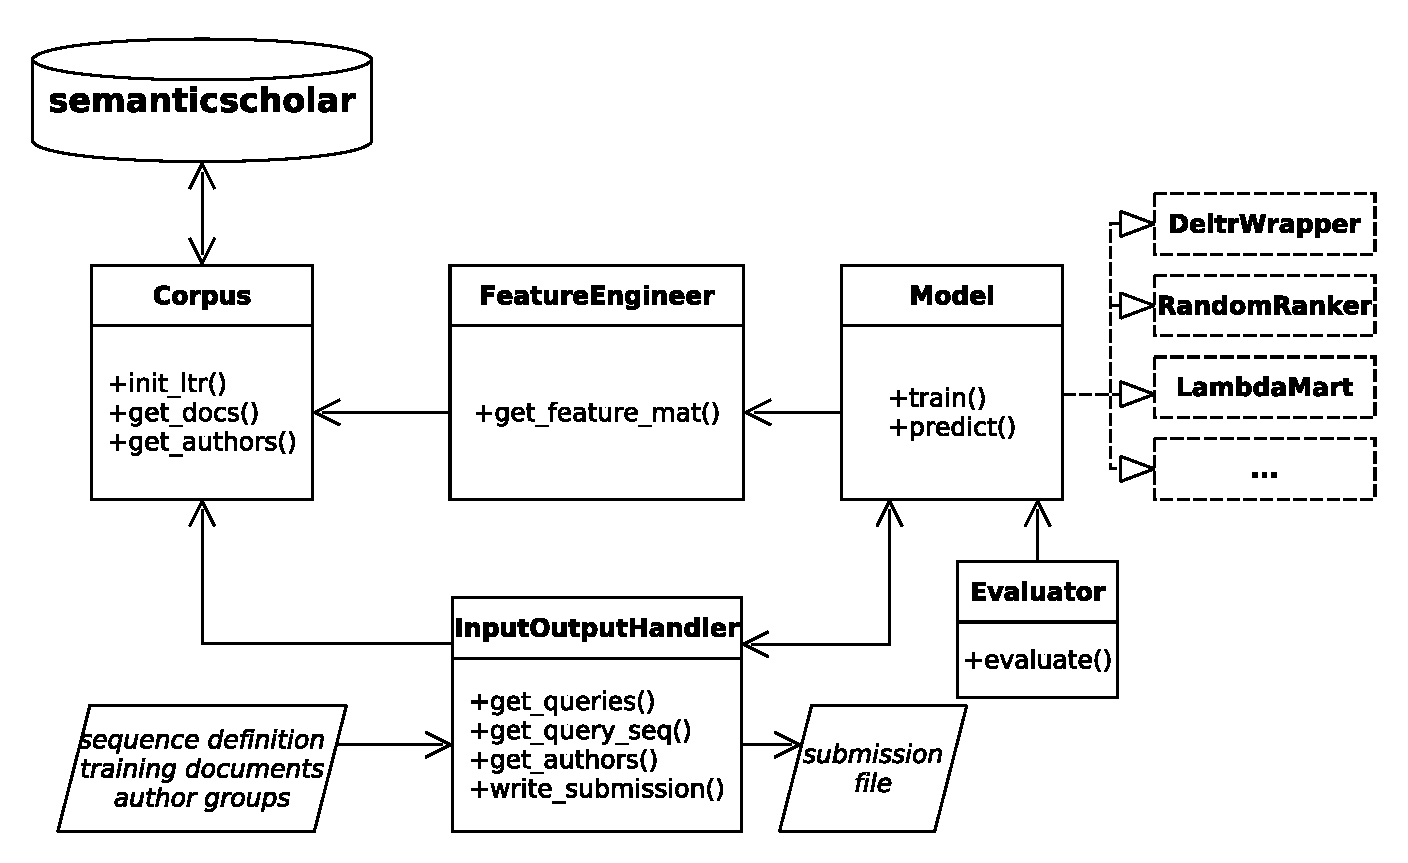
\includegraphics[width=\columnwidth]{model.pdf}
    \caption{Class diagram that describes the software modules and their dependencies.}
    \label{fig:model}
\end{figure}

\begin{table}[t]
    \centering
    \begin{tabular}{ll}
    \toprule
    level & feature \\
    \midrule
    query-document (BM25) &  title\\
    & abstract \\
    & entities \\
    & venue \\
    & journal \\
    & authors' names \\
    \midrule
    document &  year\\
    & out-citations \\
    & in-citations \\
    \midrule
    query & query length \\
    \bottomrule
    \end{tabular}
    \caption{Features used for the system}
    \label{tab:features}
\end{table}

The \emph{Model} class serves as an interface to different model implementations, and it allows for the integration of further approaches. Given a group definition, the \emph{Evaluator} class can be used to calculate the performance of a trained system in terms of searcher's relevance $U$ and author's unfairness $\Delta$. Finally, the \emph{InputOutputHandler} class is used to handle and parse the various input files and to prepare a valid output file for submission. The system accepts a list of query sequences, a list of rankings, and a partition of authors into groups. 

Some of the assessed documents were not included in the corpus and have been removed. Further, as proposed by the organizers \cite{asia_biega_trec_2019}, rankings with fewer than five entries were also removed. The removal resulted in a drop of $15\%$ of the training queries and led to roughly $3800$ documents with a relevance judgement.

\section{Results}

The test files consisted of $5$ sequences of query-ranking pairs. Each sequence had $25000$ entries, that consist of a query and a list of corresponding unlabelled documents. The query sequences were created by sampling queries with replacement from an original test set of $635$ unique queries with around $4300$ corresponding documents. The specific sampling process is not known.

The submissions' performance was assessed by calculating the aggregated relevance $U$ and the aggregated unfairness $\Delta$ based on two different author partitions: First, groups were calculated according to their productivity and impact, approximated by the h-index. And second, according to the economic level of their country of origin. Note that the group definitions were not known beforehand and were only revealed after the submission phase.  

\begin{table}[h]
    \centering
    \begin{tabular}{lccc}
    \toprule
    & \multicolumn{2}{c}{unfairness} & relevance \\
    \cmidrule(r){2-3} \cmidrule(l){4-4}
     & $\Delta_{hindex}$ & $\Delta_{level}$ & $U$  \\
    min  & 0.0405 & 0.0059 & 0.5480  \\
    mean & 0.0753 & 0.0435 & 0.6100  \\
    max  & 0.1110 & 0.0832 & 0.6740  \\
    \midrule
    random & 0.0405 & 0.0326 & 0.5480 \\
    lambdamart & 0.0855 &0.0741 & 0.6600  \\
    \bottomrule
    \end{tabular}
    \caption{Aggregated test results, averaged over the five query sequences.}
    \label{tab:results}
\end{table}

Table \ref{tab:results} summarises the aggregated performance of all submissions. For better readability, results from the five query-sequences have been averaged as we did not find any large differences between the individual sequences. 

Interestingly, our randomized submission has the lowest unfairness value for the h-index partition, and a below-average unfairness for the economic level group. It also performs worst for relevance. The second submission, the \emph{LambdaMart} algorithm, optimized users' relevance. As expected, it performed above average and achieved a relevance score close to the maximum. In terms of unfairness, this method performs above average as well but does not come close to the maximum unfairness values observed. Therefore, as this method utilizes a known learning-to-rank retrieval framework, it provides a useful baseline for both unfairness and relevance. In addition, it shows the magnitude of unfairness that current systems, which solely optimize for relevance, produce. 

\section{Discussion}

For the first Fair Ranking Track at TREC 2019, we utilized a basic learning-to-rank framework for solving this task. The main challenge was that multiple objectives (searchers' relevance and authors' group fairness) had to be optimized under the constraint of an unknown author-group-partition. This constraint seems not practicable, as one can presumably always find an arbitrary group definition that \emph{maximizes unfairness} for a given list of rankings. Existing fairness frameworks in the literature require some group definitions during training time or, for post-processing methods, the group definitions are required for re-ranking a system's output \emph{before} the final submission \cite{zehlike_fairsearch:_2019}. Further research should concentrate on first, exploring the solution space of the optimization problem and analytically study the trade-offs between high fairness and high relevance. Second, robust ranking models should be implemented. Ideally, they can be trained without requiring a specific group definition, but should later handle various group definitions when making actual ranking decisions.  


\begin{acks}
This research was supported by the Digital Society research program funded by the Ministry of Culture and Science of the German State of North Rhine-Westphalia.
\end{acks}

\bibliographystyle{ACM-Reference-Format}
\bibliography{literature}
\end{document}
